\documentclass[10pt]{beamer}

\usetheme{metropolis}
\usepackage{booktabs}
% \usepackage[scale=2]{ccicons}
\usepackage{pgfplots}
\usepackage{cancel}
\usepackage[ngerman]{babel}
\usepackage[utf8]{inputenc}
\usepackage{blindtext}
\usepackage{amsmath}
\usepackage[italicdiff]{physics}
\usepackage[italic]{hepnames}
\usepackage{graphicx}
\usepackage{float}
\usepackage{color}
\usepackage{rotating}
\usepackage{mathtools}
\usepackage{physics}
\usepackage[absolute,overlay]{textpos}
%\usepackage[texcoord,grid,gridcolor=red!10,subgridcolor=green!10,gridunit=pt]{eso-pic}

\usepackage{tikz}
\usetikzlibrary{arrows,shapes, positioning}
\usetikzlibrary{trees}
\usetikzlibrary{decorations.pathmorphing}
\usetikzlibrary{decorations.markings}
\usetikzlibrary{decorations.text}

\usepgfplotslibrary{dateplot}

% customization of mtheme

\definecolor{mDarkBrown}{HTML}{604c38}
\definecolor{mDarkTeal}{HTML}{23373b}
\definecolor{mLightBrown}{HTML}{EB811B}
\definecolor{mLightGreen}{HTML}{14B03D}

\setbeamercolor{frametitle}{use=structure, parent=structure}
  \setbeamercolor{normal text}{%
    fg=black!80,
    bg=white
  }
% Frontpage
\title{ENERGY REGRESSION WITH DEEP LEARNING IN PARTICLE COLLIDER PHYSICS}
\date{\today}
\author{Simon Schnake}
\institute{Universität Hamburg}

%%% make red todo notes
\newcommand{\todo}[1]{\textcolor{red}{TODO: #1}\PackageWarning{TODO:}{#1!}}

% Document

\begin{document}

\maketitle
\tikzstyle{every picture}+=[remember picture]
\tikzstyle{na} = [baseline=-.5ex]

\begin{frame}{Flow of Content}
  \todo{Ablaufplan}
\end{frame}

\section{Toy Calorimeter Analysis}

\begin{frame}{Calorimetry}
  \begin{columns}
    \column{0.65\textwidth}
    \begin{itemize}
    \item leading processes in shower development
      \begin{itemize}
      \item bremsstrahlung
      \item pair production
      \end{itemize}
    \item measure the energy of the particle shower (destructive)
    \item resolution of a calorimeter
      $\frac{\sigma}{E} = \frac{a}{\sqrt{E}} \otimes b \otimes \frac{c}{E} $
    \end{itemize}
    \column{0.5\textwidth}
    \begin{figure}[htp]
      \tikzset{
        photon/.style={decorate, decoration={snake}, draw=red},
        electron/.style={draw=black}
      }

      \begin{tikzpicture}[
        thick,
        % Set the overall layout of the tree
        level/.style={level distance=1.5cm},
        level 2/.style={sibling distance=2.6cm},
        level 3/.style={sibling distance=3.2cm}
        ]

        \filldraw[fill=brown!20!white, draw=black] (0.5, 1.75) rectangle (4.5,-3.5);
        \filldraw[fill=brown!30!white, draw=brown!30!white] (1.0, 1.70) rectangle (1.5, -3.45);
        \filldraw[fill=brown!30!white, draw=brown!30!white] (2.0, 1.70) rectangle (2.5, -3.45);
        \filldraw[fill=brown!30!white, draw=brown!30!white] (3.0, 1.70) rectangle (3.5, -3.45);
        \filldraw[fill=brown!30!white, draw=brown!30!white] (4.0, 1.70) rectangle (4.45, -3.45);
        
        \draw[electron] (0,0) -- (1,0);
        \draw (-0.15, 0.1) node {$e^{-}$};
        \draw[photon] (1,0) -- (1.7, -1.25);
        \draw[electron] (1,0) -- (2, 0.55);
        \draw[electron] (1.7, -1.25) -- (2.5, -1);
        \draw[electron] (1.7, -1.25) -- (2.5, -2.05);
        \draw[electron] (2, 0.55) -- (2.7, 0);
        \draw[photon] (2, 0.55) -- (3, 0.75);
        \draw[photon] (2.5, -2.05) -- (3.1, -2.);
        
        \draw[electron] (3, 0.75) -- (3.7, 1.25);
        \draw (3.95, 1.35) node {$e^{-}$};
        \draw[electron] (3, 0.75) -- (3.7, 0.45);
        \draw (3.95, 0.5) node {$e^{+}$};
        \draw[photon] (2.7, 0) -- (3.7, 0.1);
        \draw (3.85, 0.1) node {$\gamma$};
        \draw[electron] (2.7, 0) -- (3.7, -0.5);
        \draw (3.95, -0.4) node {$e^{-}$};
        \draw[electron] (2.5, -1) -- (3.7, -0.8);
        \draw (3.95, -0.75) node {$e^{-}$};
        \draw[photon] (2.5, -1) -- (3.7, -1.2);
        \draw (3.85, -1.2) node {$\gamma$};
        \draw[electron] (3.1, -2.) -- (3.7, -1.5);
        \draw (3.95, -1.4) node {$e^{+}$};
        \draw[photon] (3.3, -2.15) -- (3.7, -2);
        \draw (3.85, -2) node {$\gamma$};

        \draw[electron] (3.1, -2.) -- (3.7, -2.5);
        \draw (3.95, -2.45) node {$e^{-}$};
        \draw[electron] (2.5, -2.05) -- (3.7, -3.);
        \draw (3.95, -2.95) node {$e^{+}$};
      \end{tikzpicture}
    \end{figure}
  \end{columns}
\end{frame}


\begin{frame}{Simulation Setup}
  \begin{textblock*}{220pt}(150pt, 40pt)
    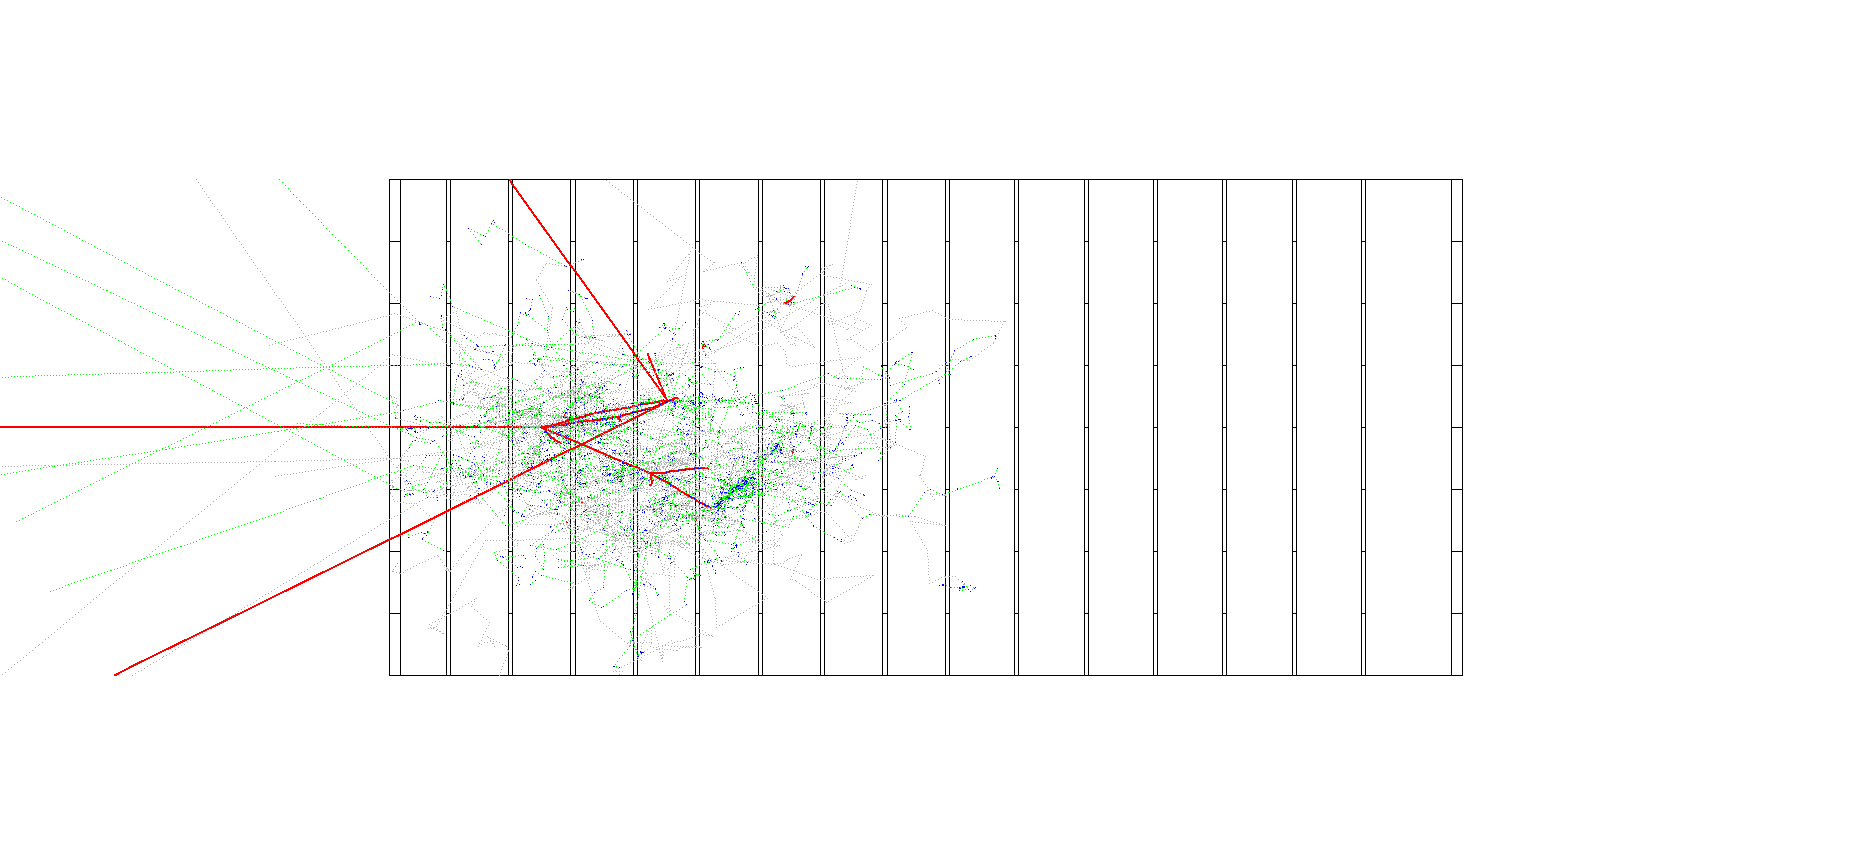
\includegraphics[width=\textwidth]{../images/side.png}
  \end{textblock*}
  \begin{textblock*}{150pt}(2pt,100pt)
    \begin{itemize}
    \item Simulation with Geant4\small{}
    \item $e^-$ from 0. to 10 GeV
    \item 300,000 events
    \item 8x8x17 (1088) scint cells
    \item measure charged tracks in each scintillator cell
    \end{itemize}
  \end{textblock*}
  \begin{textblock*}{10pt}(170pt,150pt)
    \begin{tabular}{l|l|l}
      layer  & scint    & absorber \\ \hline
      layer 0      & 9mm     & 40 mm steel\\
      layer 1 - 8  & 3.7mm   & 50.5 mm brass \\
      layer 9 - 14 & 3.7mm   & 56.5 mm brass \\
      layer 15     & 3.7 mm  & 75 mm steel\\
      layer 16     & 9mm     &                      
    \end{tabular}
  \end{textblock*}
\end{frame}

\begin{frame}{Resulting Data}
\centering  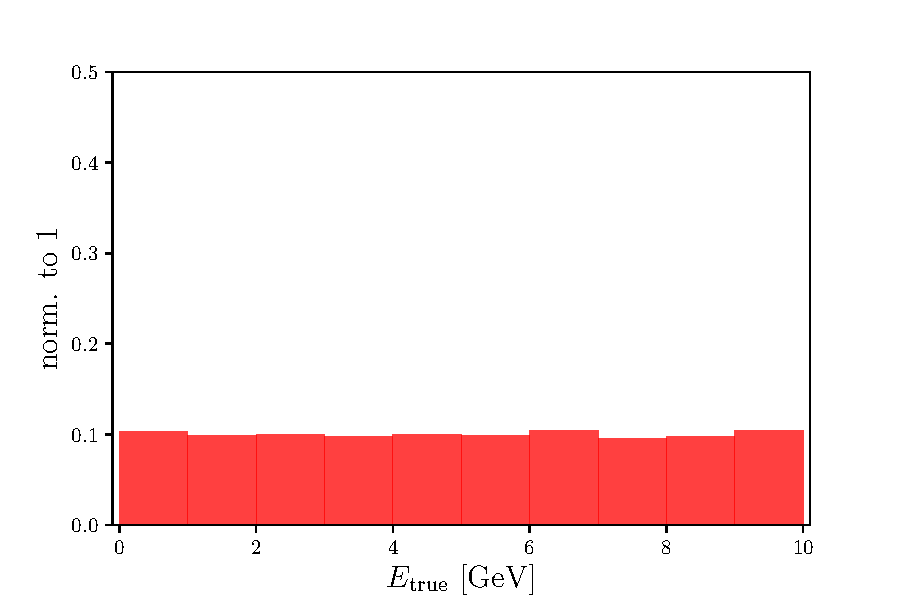
\includegraphics[width=0.51 \textwidth]{../images/energy_distribution.pdf}
  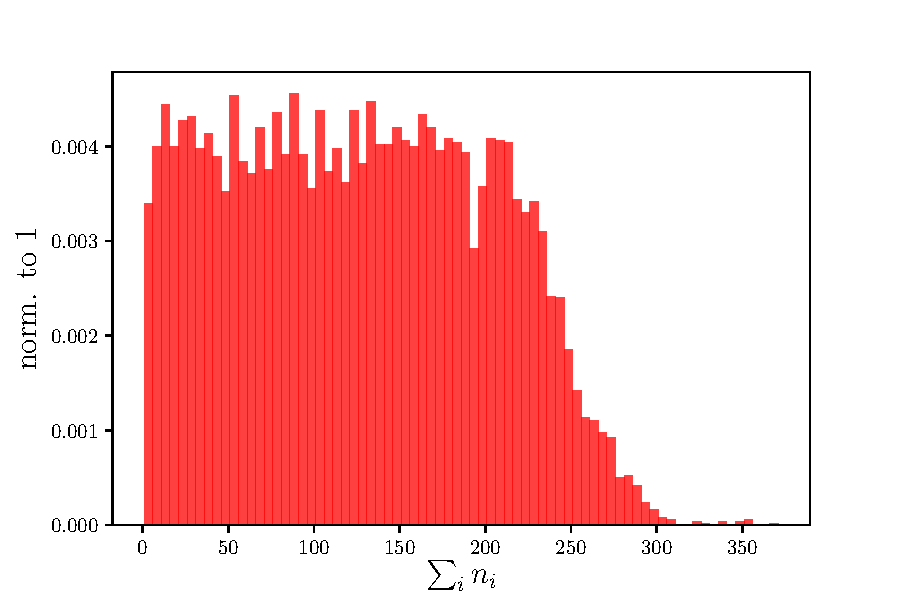
\includegraphics[width=0.49 \textwidth]{../images/sumn_distribution.pdf}
  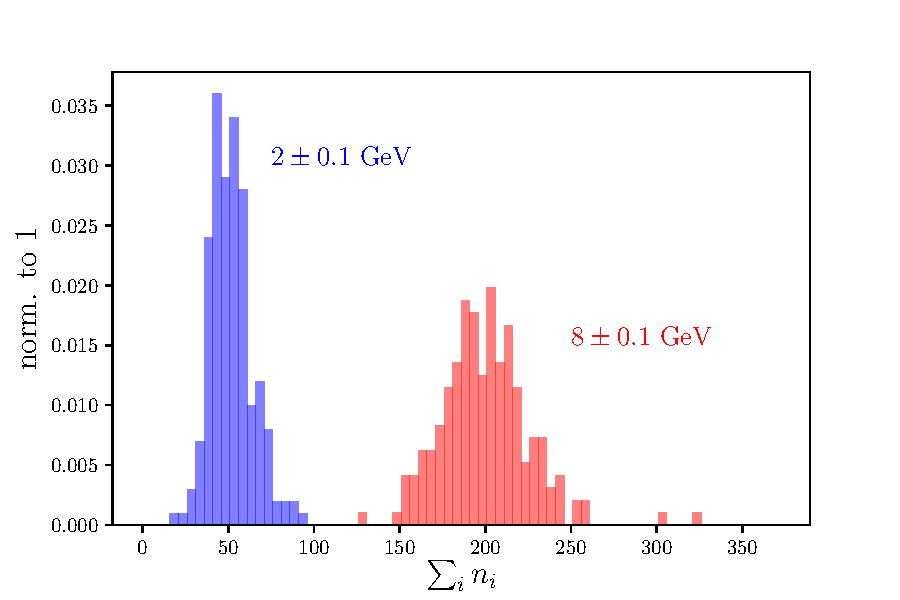
\includegraphics[width=0.49 \textwidth]{../images/sumn_e28_distribution.pdf}
\end{frame}

\begin{frame}{Resulting Data}
  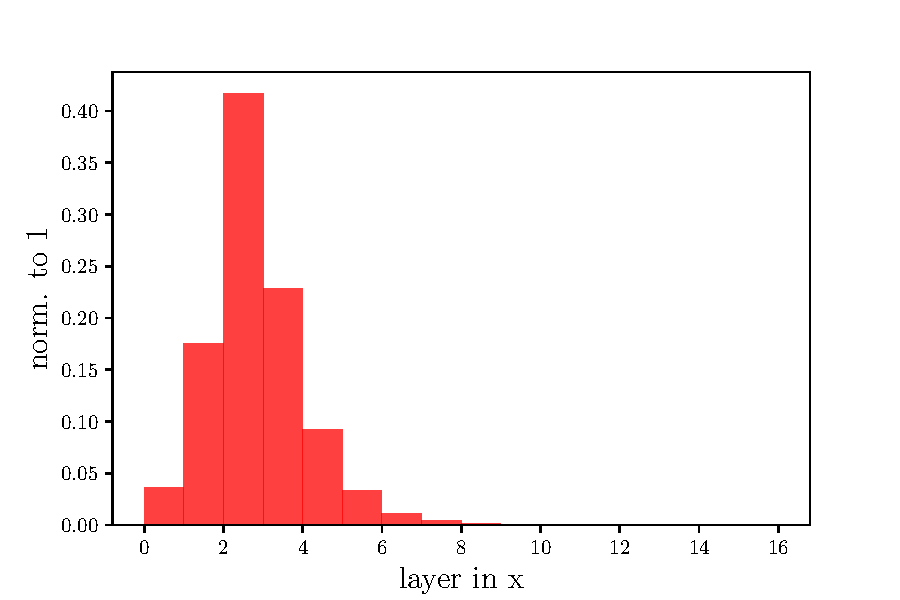
\includegraphics[width=0.49 \textwidth]{../images/x_distribution.pdf}
  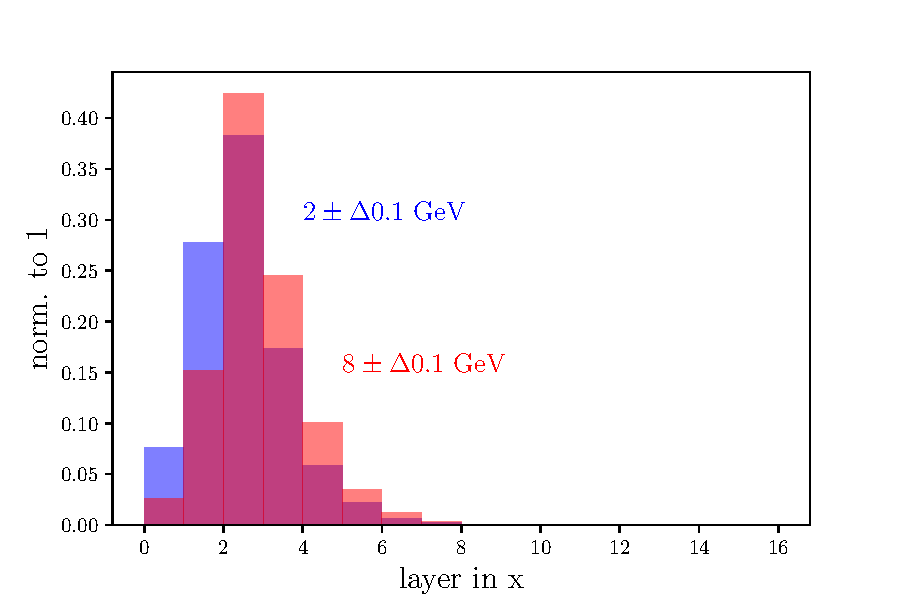
\includegraphics[width=0.49 \textwidth]{../images/x_e28_distribution.pdf}
  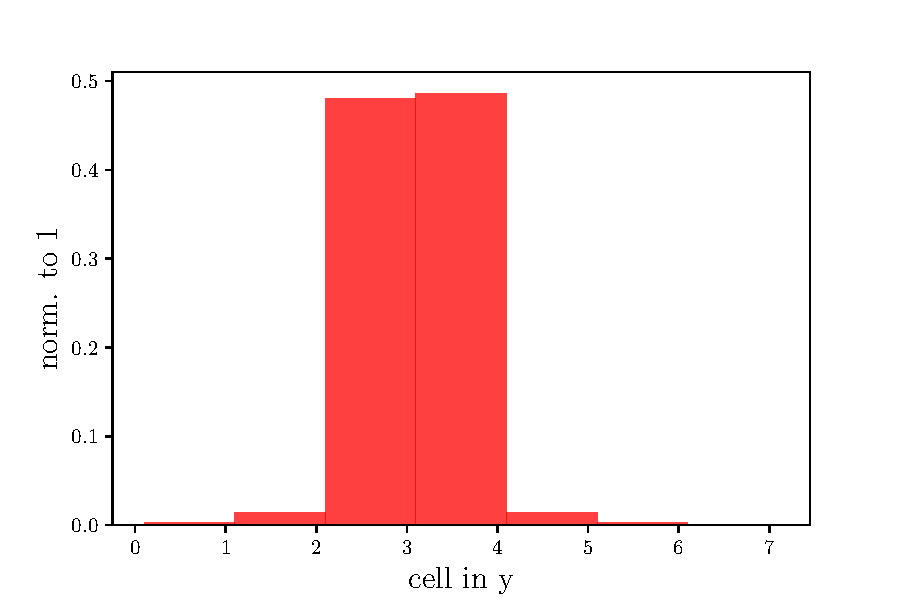
\includegraphics[width=0.49 \textwidth]{../images/y_distribution.pdf}
  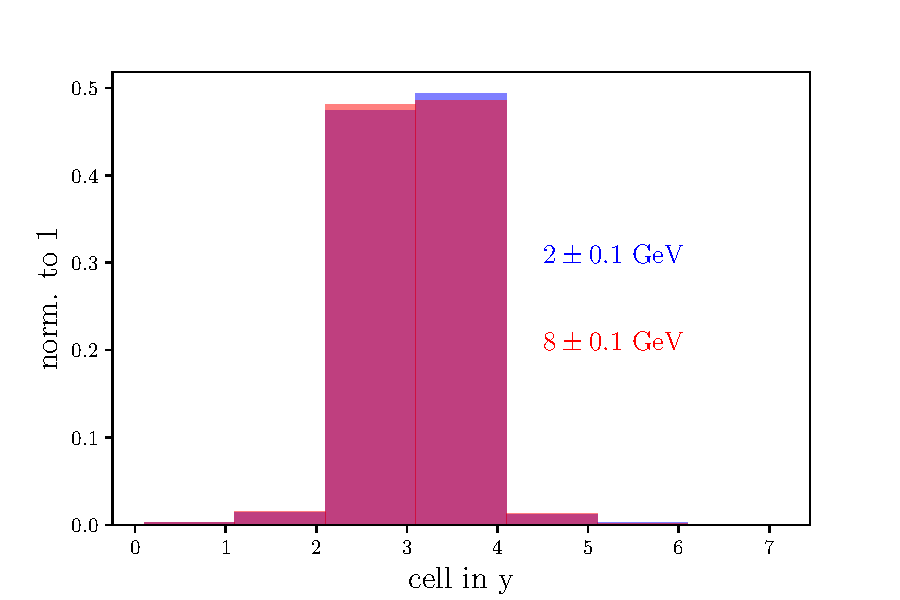
\includegraphics[width=0.49 \textwidth]{../images/y_e28_distribution.pdf}
\end{frame}

\begin{frame}{Resulting Data}
    \begin{textblock*}{250pt}(20pt, 75pt)
    Calibration by linear fitting:
  \end{textblock*}
  \begin{textblock*}{150pt}(150pt, 20pt)
    \begin{figure}[htp]
      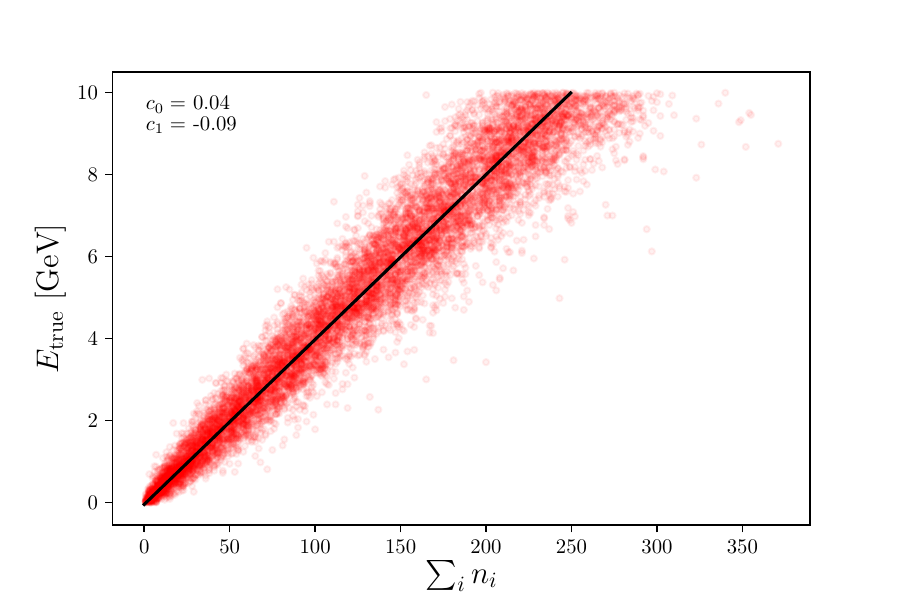
\includegraphics[width=\textwidth]{../images/e-vs-sum_n_fit.png}
    \end{figure}
  \end{textblock*}
  \begin{textblock*}{250pt}(20pt, 175pt)
    Visualization of the data:
  \end{textblock*}
  \begin{textblock*}{135pt}(150pt, 120pt)
    \begin{figure}[htp]
      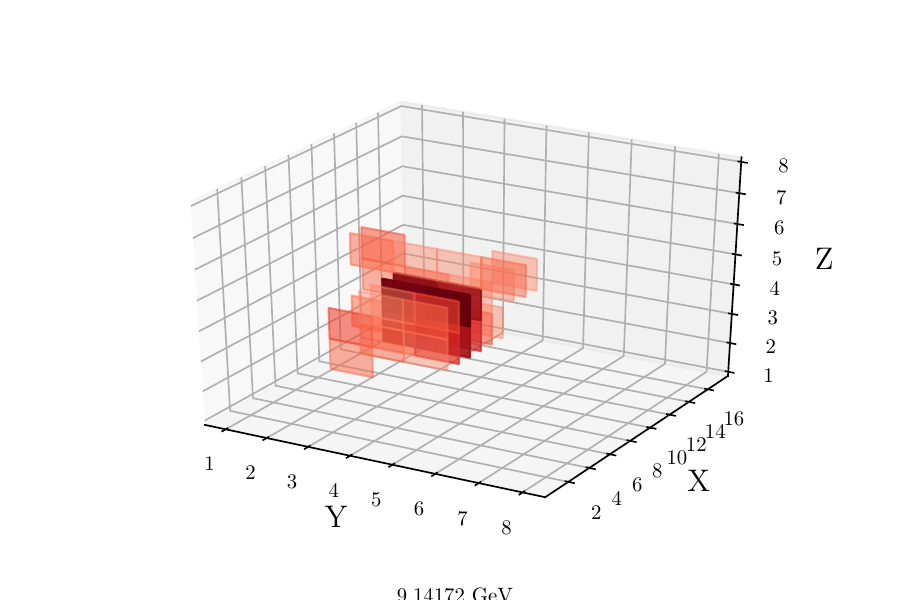
\includegraphics[width=1.1\textwidth]{../images/data_display.png}
    \end{figure}
  \end{textblock*}
\end{frame}

\begin{frame}{Deep Learning}
  \begin{textblock*}{150pt}(200pt,35pt)
    \begin{figure}[htp]
      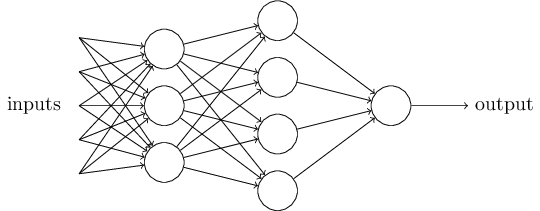
\includegraphics[width=\textwidth]{../images/tikz1.png}
    \end{figure}
  \end{textblock*}
  \begin{textblock*}{150pt}(215pt,155pt)
    \Huge{$\}$}
  \end{textblock*}
  \begin{textblock*}{150pt}(230pt,164pt)
    \emph{Backpropagation}
  \end{textblock*}
  \begin{itemize}
  \item Pass input $X$ to the network
  \item Calculate output $\hat{Y}$ and difference\\ to true value $Y$ (loss function)
  \item Minimize loss function:
    \begin{itemize}
    \item Calculate gradient of the loss
    \item Use gradient to update weights $W, b$
    \end{itemize}
  \end{itemize}
  \begin{textblock*}{150pt}(20pt,200pt)
    \begin{align*}
      &a^{[0]} \coloneqq X \\
      &a^{[l]} \coloneqq \sigma^{[l]}(W^{[l]} a^{[l-1]}+ b^{[l]})\\
      &\hat{Y}(X) \coloneqq a^{[L]}
    \end{align*}
  \end{textblock*}

  \begin{textblock*}{170pt}(160pt,210pt)
    \begin{align*}
      &\text{\emph{Example Loss}:}\\
      &\mathcal{L}(\hat{Y}, Y) = (\hat{Y} - Y)^2
    \end{align*}
  \end{textblock*}
\end{frame}

\begin{frame}{Deep Learning Model}
  \centering
  \begin{tabular}{l|l|l|l|l}
    Layer & Type  & Activation & Output Shape & \# Parameter \\
    \hline
    0     & Input &            & (8, 8, 17, 1) &  \\
    1   & Conv3D(32, (3,3,3)) & ReLU & (8, 8, 17, 32)   & 896   \\
    2   & Conv3D(10, (3,3,3)) & ReLU & (6, 6, 15, 10)   & 8650  \\
    3   &  Conv3D(5, (5, 5, 5)) & ReLU & (2, 2, 11, 5)  & 6255  \\
    4     & Flatten()  & & 220 &               \\
    5   & Dense(128)                          & ReLU & 128 & 28288          \\
    6-7 & Dense(128)  & ReLU & 128 & 16512 \\
    8     & Dense(10)                           & ReLU & 10 & 1290         \\
    10     & Dense(1)                            & Linear   & 1 & 11 
  \end{tabular}
  \begin{itemize}
  \item Loss = mean squared error
  \item Optimizer = RMSprop
  \item Data Augmentation with symmetry transformation (flipping, rotating and shifting)
  \end{itemize}
\end{frame}

\begin{frame}{First Results}
  \begin{columns}
    \column{0.5\textwidth}
    \begin{figure}[htp]
      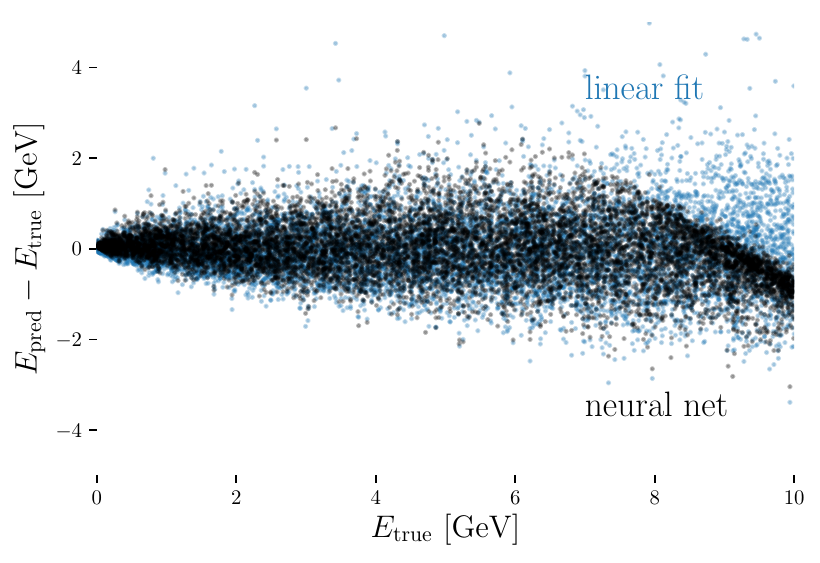
\includegraphics[width=1.1\textwidth]{../images/data_augment.png}
    \end{figure}
    \column{0.5\textwidth}
    \begin{figure}[htp]
      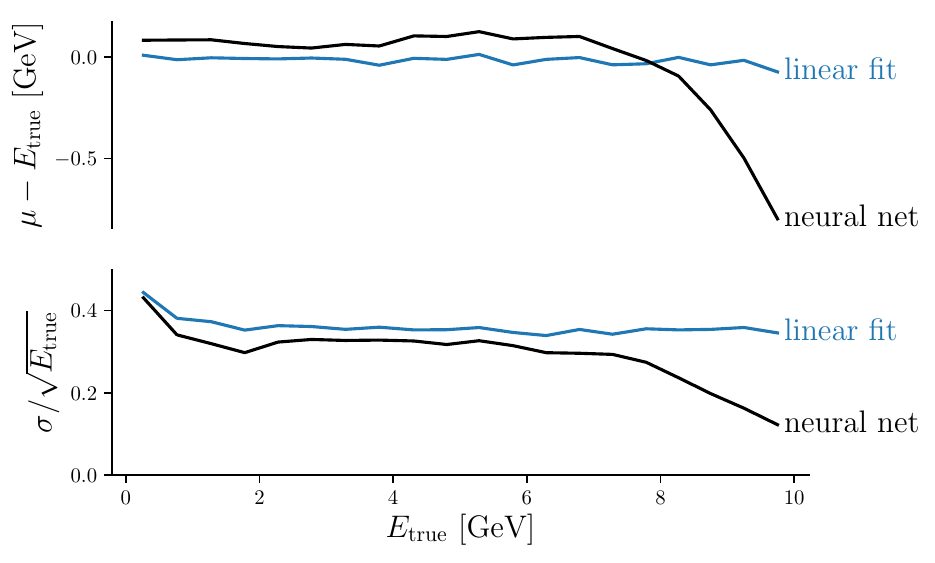
\includegraphics[width=1.1\textwidth]{../images/data_augment_res.png}
    \end{figure}
  \end{columns}


  \begin{textblock*}{150pt}(100pt,90pt)
    \tikz[na] \node[coordinate] (n1) {};
  \end{textblock*}
  \begin{textblock*}{150pt}(250pt,90pt)
    \tikz[na] \node[coordinate] (n2) {};
  \end{textblock*}
  \begin{tikzpicture}[overlay]
    \draw<1> [blue, thick, ->] (n1) to [bend left=30] node [above, sloped] (text) {binned statistics} (n2);
  \end{tikzpicture}
 
  % description kink
  \begin{textblock*}{150pt}(70pt, 210pt)
    \only<2->{Problems:}
    \begin{itemize}
    \item<2-> kink in distribution \tikz[na] \node[coordinate] (kink) {};
    \item<2-> shift to higher values \tikz[na] \node[coordinate] (shift) {};
    \end{itemize}
  \end{textblock*}
  % kink point scatter plot
  \begin{textblock*}{150pt}(170pt,135pt)
    \tikz[na] \node[coordinate] (p1) {};
  \end{textblock*}
  % kink point quant plot
  \begin{textblock*}{150pt}(330pt,130pt)
    \tikz[na] \node[coordinate] (p2) {};
  \end{textblock*}
  % shift point
  \begin{textblock*}{150pt}(280pt,102pt)
    \tikz[na] \node[coordinate] (p3) {};
  \end{textblock*}
  \begin{tikzpicture}[overlay]
    \path[red, thick, ->]<2> (kink) edge [bend right] (p1);
    \path[red, thick, ->]<2> (kink) edge [bend right] (p2);
    \path[red, thick, ->]<3> (shift) edge [bend right=80] (p3);
  \end{tikzpicture}
\end{frame}

\begin{frame}{Adversarial Training}
    \centering
  \usetikzlibrary{arrows}
  \def\layersep{1cm}
    \small
    \begin{tikzpicture}[shorten >= 1pt, ->, node distance=\layersep,scale=.50]
      \tikzstyle{neuron} = [circle, minimum size=0.25cm, draw=black!20, line width=0.3mm, fill=white]

      % Classifier f
      \node at (2,0) {Classifier $f$};
      \draw (-1,-0.5) rectangle (4,-5.5);

      \path[->, shorten >= 0pt] (-2,-3) edge (-1,-3);
      \node[left] at (-2,-3) {$X$};

      \path[-o, shorten >= 0pt] (1.5,-6.5) edge (1.5,-5.5);
      \node[below] at (1.5,-6.5) {$\theta_f$};

      \path[->, shorten >= 0pt] (3.5,-3) edge (6.5,-3);
      \node[above] at (5.25,-3) {$f(X;\theta_f)$};

      \path[dashed,-] (5.25,-3) edge (5.25,-6.5);
      \node[below] at (5.25,-6.5) {${\cal L}_f(\theta_f)$};

      \foreach \name / \y in {1,...,3}
      \node[neuron] (f-I-\name) at (-0.5,-1-\y) {};

      \foreach \name / \y in {1,...,5}
      \node[neuron] (f-H1-\name) at (-0.5cm+\layersep,-\y cm) {};
      \foreach \name / \y in {1,...,5}
      \node[neuron] (f-H2-\name) at (-0.5cm+3*\layersep,-\y cm) {};

      \node[neuron] (f-O) at (-0.5cm+4*\layersep,-3cm) {};

      \foreach \source in {1,...,3}
      \foreach \dest in {1,...,5}
      \path[black] (f-I-\source) edge (f-H1-\dest);

      \foreach \source in {1,...,5}
      \path[black] (f-H2-\source) edge (f-O);

      \node[black] at (1.5,-3) {...};

      % Adversary r
      \node at (9,0) {Adversary $r$};
      \draw (6.5,-0.5) rectangle (11.5,-5.5);

      \node[above] at (14,-3) {$r(f(X;\theta_f);\theta_r)$};
      \path[-o, shorten >= 0pt] (11,-3) edge (15,-3);
      \path[-o, shorten >= 0pt] (9,-6.5) edge (9,-5.5);
      \node[below] at (9,-6.5) {$\theta_r$};

      \foreach \name / \y in {1,...,1}
      \node[neuron] (r-I-\name) at (7,-2-\y) {};

      \foreach \name / \y in {1,...,5}
      \node[neuron] (r-H1-\name) at (7cm+\layersep,-\y cm) {};
      \foreach \name / \y in {1,...,5}
      \node[neuron] (r-H2-\name) at (7cm+3*\layersep,-\y cm) {};

      \node[neuron] (r-O1) at (7cm+4*\layersep,-2cm) {};
      \node[neuron] (r-O2) at (7cm+4*\layersep,-3cm) {};
      \node[neuron] (r-O3) at (7cm+4*\layersep,-4cm) {};

      \foreach \source in {1,...,1}
      \foreach \dest in {1,...,5}
      \path[black] (r-I-\source) edge (r-H1-\dest);

      \foreach \source in {1,...,5}
      \path[black] (r-H2-\source) edge (r-O1);
      \foreach \source in {1,...,5}
      \path[black] (r-H2-\source) edge (r-O2);
      \foreach \source in {1,...,5}
      \path[black] (r-H2-\source) edge (r-O3);

      \node[black] at (9,-3) {...};

      \draw[dashed,-] (14.9,-6.5) -- (14.9,-3);
      \node[below] at (15,-6.5) {${\cal L}_r(\theta_f, \theta_r)$};
    \end{tikzpicture}

    \footnotesize{\color{gray} G. Louppe, "Learning to Pivot with Adversarial Networks", 1611.01046} \\
  Procedure:
  \begin{itemize}
  \item Pretrained Classifier
  \item Train Adversarial with  $ {\cal L}_r(\theta_f, \theta_r)$
  \item Train Classifier with $ E_\lambda(\theta_f, \theta_r) = {\cal L}_f(\theta_f) - \lambda {\cal L}_r(\theta_f, \theta_r)$ 
  \item repeat last two steps until convergence
  \end{itemize}

\end{frame}

\begin{frame}{Adversarial Training}
  \begin{itemize}
  \item Results after training $i \cdot$ 5 epochs each network
  \end{itemize}
  \begin{figure}[hbtp]
    \centering
    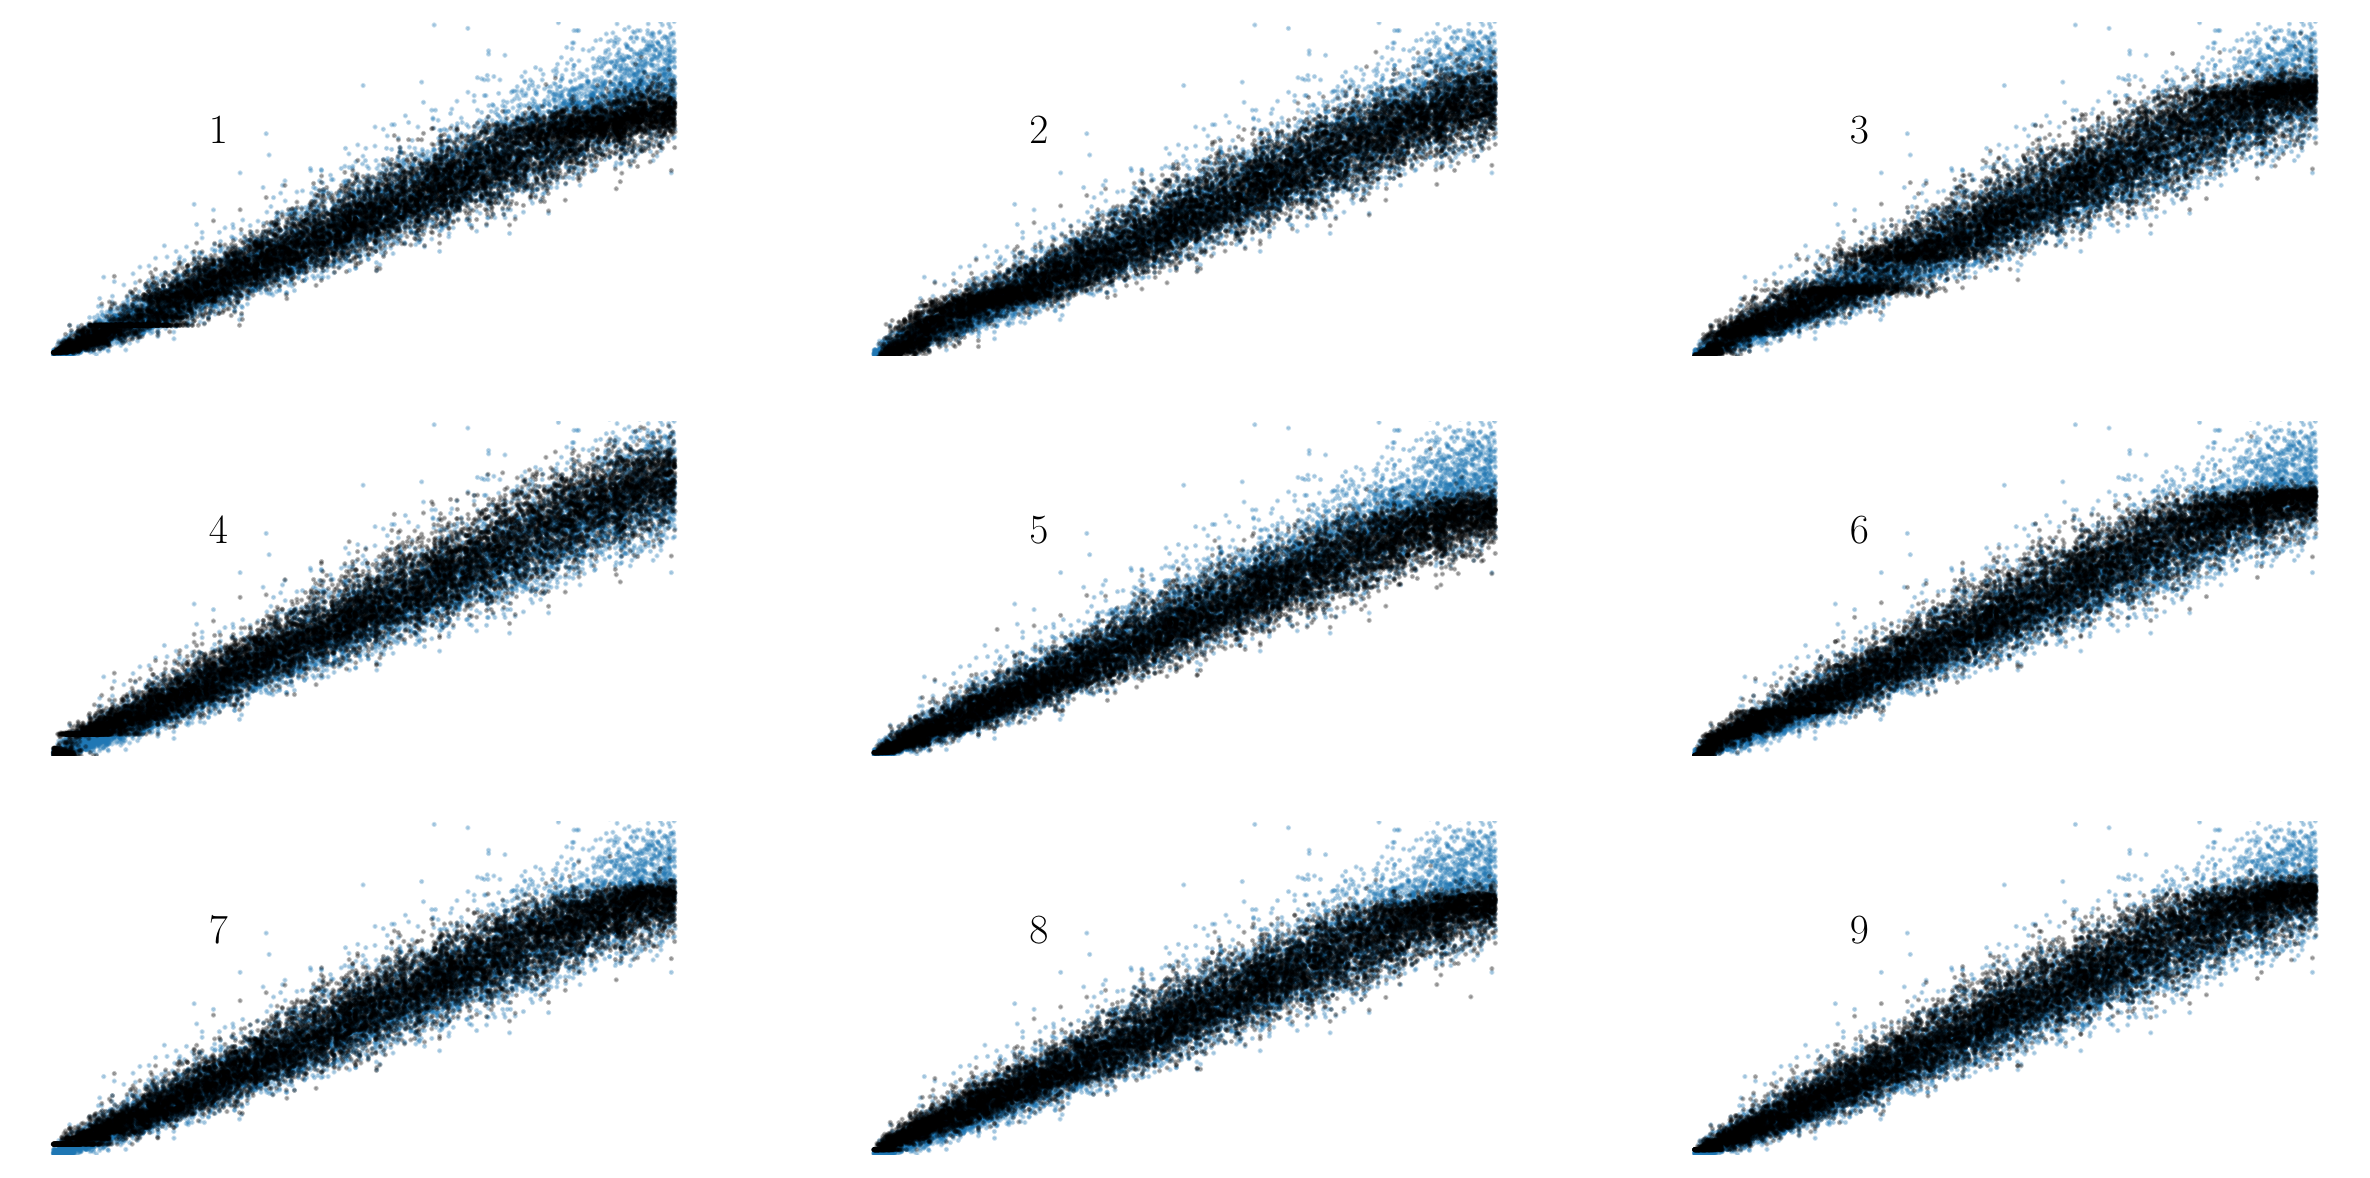
\includegraphics[width=.9\linewidth]{../images/adv_scatter.png}
  \end{figure}
  \begin{itemize}
  \item No Convergence
  \end{itemize}
\end{frame}

\begin{frame}{Maximum Likelihood Loss}
  \begin{align*}
    &\text{min} \sum (y_{\text{true}}-y_{\text{pred}})^2 \\
    =&\text{max} \sum\frac{-(y_{\text{true}}-y_{\text{pred}})^2}{2 \sigma^2} - \ln(\sqrt{2\pi \sigma^2}) \\
    = &\text{max} \sum \ln(\exp(-\frac{(y_{\text{true}}-y_{\text{pred}})^2}{2 \sigma^2})) - \ln(\sqrt{2\pi \sigma^2}) \\
    = &\text{max} \sum \ln( \frac{1}{\sqrt{2\pi \sigma^2}} e^{-\frac{(y_{\text{true}}-y_{\text{pred}})^2}{2 \sigma^2}}) \\
    = &\text{max} \ln \prod \frac{1}{\sqrt{2\pi \sigma^2}} e^{-\frac{(y_{\text{true}}-y_{\text{pred}})^2}{2 \sigma^2}}
  \end{align*}
    By using the mean squared error as a loss function we imply that our values are gaussian distributed with constand $\sigma$
\end{frame}

\begin{frame}{Maximum Likelihood Loss}

  \begin{textblock*}{150pt}(10pt, 55pt)
    \begin{itemize}
    \item Toy Gaussian Monte Carlo
    \item Max Likelihood Fit \emph{\textcolor{black}{Gaussian}} and \emph{\textcolor{blue}{Normed Gaussian}}
    \end{itemize}
  \end{textblock*}

  
  \begin{textblock*}{150pt}(175pt,35pt)
      \includegraphics[width=\textwidth]{../images/gaussian_cut.pdf}
  \end{textblock*}

  \begin{textblock*}{150pt}(5pt,140pt)
    \begin{align*}
      &\text{max log likelihood} = -\text{min} \sum \ln(\frac{\text{Norm}(y_{\text{true}} | y_{\text{pred}}, \sigma)}{\int^b_a \text{Norm}(y_{\text{true}} | y_{\text{pred}}, \sigma)})\\ \\
                                            &=\ \text{min} \sum \underbrace{\frac{(y_{\text{true}}-y_{\text{pred}})^2}{\sigma^2}}_{\text{\textcolor{blue}{mean squared weighted error}}} +\underbrace{\ln(\frac{\pi \sigma^2}{2} \left(\text{erf}(\frac{y_{\text{pred}}-a}{\sqrt{2}\sigma}) - \text{erf}(\frac{y_{\text{pred}}-b}{\sqrt{2}\sigma})\right)^2)}_{\text{\textcolor{red}{boundary correction term}}}
    \end{align*}
  \end{textblock*}

\end{frame}

\begin{frame}{Maximum Likelihood Loss}
  \begin{itemize}
  \item Start with pretrained model
  \item Train network with loss from last slide and $\sigma = 0.31 \sqrt{y_{\text{true}}}$
  \end{itemize}
  \begin{columns}
    \column{0.5\textwidth}
    \begin{figure}[htp]
      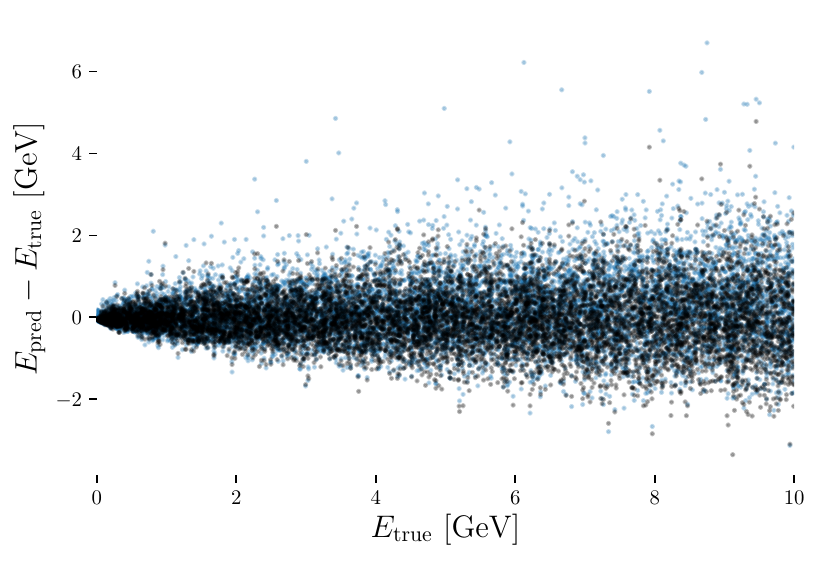
\includegraphics[width=1.1\textwidth]{../images/likelihood.png}
    \end{figure}
    \column{0.5\textwidth}
    \begin{figure}[htp]
      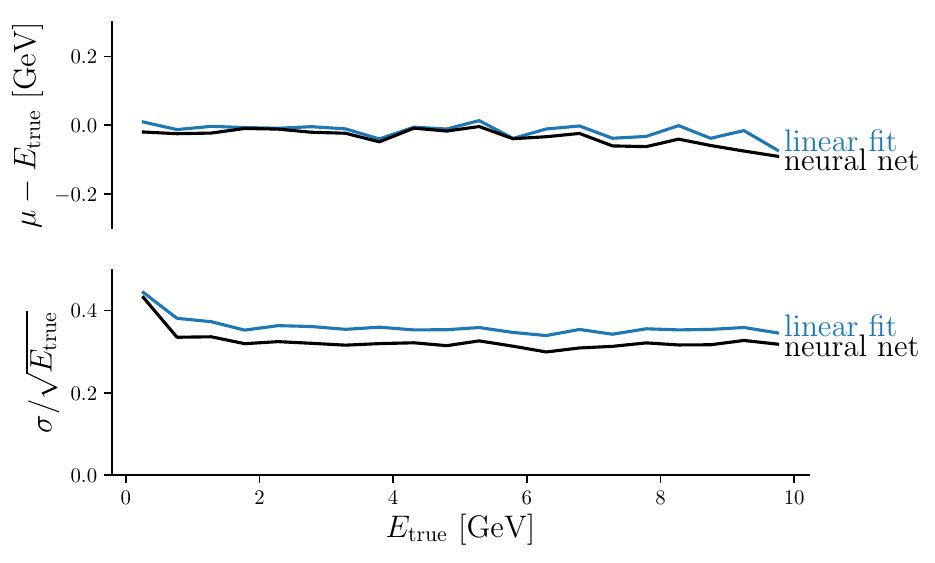
\includegraphics[width=1.1\textwidth]{../images/likelihood_res.png}
    \end{figure}
  \end{columns}

  \begin{itemize}
  \item Compensation for shift and boundary kink
  \item Network performs $\approx 10\%$ better than the linear fit 
  \end{itemize}
  
\end{frame}



\section{Jet Calibration}

\begin{frame}{QCD Jet CMS Simulation}
  \todo{Simulation vorstellen}
  \todo{Dataset vorstellen}
\end{frame}

\begin{frame}{Particle Flow Network}
  \begin{figure}[ht]
    \centering
    \includegraphics[width=0.75\textwidth]{../images/EFNDiagram.jpg}
  \end{figure}

  \footnotesize{\color{gray} {P. T. Komiske, E.M. Metodiev, and
      J. Thaler, Energy Flow Networks: Deep Sets for Particle Jets,
      JHEP 01 (2019)}}
\end{frame}

\begin{frame}{Binned Loss}
  
\end{frame}

\begin{frame}{Training Setup}
  \tikzset{
    %Define standard arrow tip
    >=stealth',
    %Define style for boxes
    punkt/.style={
      rectangle,
      draw=black, thick,
      text width=6.5em,
      minimum height=2em,
      text centered},
    % Define arrow style
    pil/.style={
      ->,
      thick,
      shorten <= 2pt,
      shorten >= 2pt},
  }

  \begin{textblock*}{250pt}(0pt, 20pt)
  \begin{figure}[htp]
    \tikzstyle{arrow} = [draw, -latex']
    \begin{tikzpicture}[]
      \node[punkt] (model) {Model};
      \node[below=2.5cm of model] (1loss) {$\mathcal{L}_{J}(P_{T,\text{Pred}}, P_{T,\text{Gen}}, \sigma)$};
      \node[below=0.3 cm of 1loss] (1st) {1st};
      \node[left=1.2cm of 1loss] (mseloss) {$(P_{T,\text{Pred}}-P_{T,\text{Gen}})^2$};
      \node[below=0.3 cm of mseloss] (mse) {MSE};
      \node[right=1.2cm of 1loss] (2loss) {$\mathcal{L}_{J}(P_{T,\text{Pred}}, P_{T,\text{Gen}}, \sigma)$};
      \node[below=0.3 cm of 2loss] (2nd) {2nd};

      \node[left=0.3 cm of mseloss] (l) {Loss:};
      
      \path [arrow, thick] (mseloss) -- (model.south west);
      \path [postaction={decorate,decoration={text along path,text
            align=center, text={train}}}] (mseloss) -- (model.south west);
      
      \path [arrow, thick] (model.south west) -- (1loss);
      \path [postaction={decorate,decoration={text along path,text
            align=center, text={predict {$\sigma$}}}}] (model.south west) -- (1loss);

      \path [arrow, thick] (1loss)  --  (model.south);
      \path [postaction={decorate,decoration={text along path,text
            align=center, text={train}}}] (1loss)  --  (model.south);
      
      \path [arrow, thick] (model.south) -- (2loss);
      \path [postaction={decorate,decoration={text along path,text
            align=center, text={predict {$\sigma$}}}}] (model.south) -- (2loss);

      \path [arrow, thick] (2loss)  --  (model.south east);
      \path [postaction={decorate,decoration={text along path,text
            align=center, text={train}}}]  (model.south east) -- (2loss);
    \end{tikzpicture}
  \end{figure}
  \end{textblock*}
  
  \begin{textblock*}{250pt}(15pt, 190pt)
    \begin{align*}
      \mathcal{L}_J=\underbrace{\frac{(P_{T,\text{Gen}}-P_{T,\text{Pred}})^2}{\sigma^2}}_{\text{\textcolor{blue}{mean squared weighted error}}} +\underbrace{\ln(\frac{\pi \sigma^2}{2} \left(\text{erf}(\frac{P_{T,\text{Pred}}-a}{\sqrt{2}\sigma}) - \text{erf}(\frac{P_{T,\text{Pred}}-b}{\sqrt{2}\sigma})\right)^2)}_{\text{\textcolor{red}{boundary correction term}}}
    \end{align*}
  \end{textblock*}
\end{frame}

\begin{frame}{Predict $\sigma$}

  \begin{itemize}
  \item Output $P_{T,\text{Pred}}$ of the network
  \item Calculate \emph{std} for $P_{T,\text{Pred}}$ sliced in 50 bins
  \end{itemize}  
 
  \begin{figure}[hbtp]
    \centering
    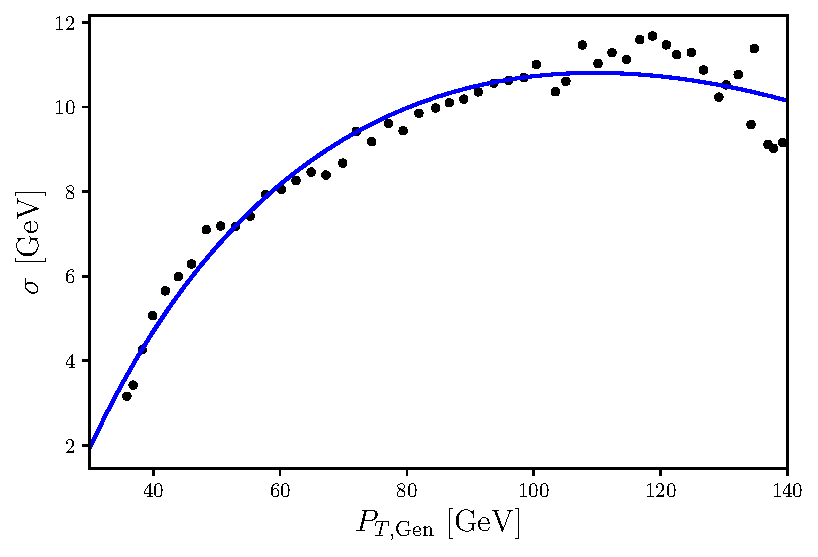
\includegraphics[width=.7\linewidth]{../images/sigma_fit.pdf}
  \end{figure}
\begin{itemize}
\item Fit \(\sigma(P_{T,\text{Gen}})= c_0 \sqrt{P_{T,\text{Gen}}}+c_1 P_{T,\text{Gen}} + c_2 \)
\item  \(\sigma(P_{T,\text{Gen}}) \) needs to be analytical for the \emph{backpropagation}
\end{itemize}  
\end{frame}

\begin{frame}{Summary and Outlook}
    Summary:
  \begin{itemize}
  \item Simulation of a calorimeter
  \item Presentation of two problems
  \item Adversarial Training
  \item Develop a customized loss function
  \end{itemize}
  Outlook:
  \begin{itemize}
  \item Simulation of pions and other particles
  \item Compare different architectures and hyperparameter tuning
  \item Energy calibration for jets
  \end{itemize}
  \only<2>{  
    \begin{textblock*}{250pt}(45pt,35pt)
      \rotatebox{-45}{\color{blue}{\Huge Thank you for your attention}}
    \end{textblock*}
  }
\end{frame}

\end{document}
